% For Campus GroepT use the two-column paper layout
\documentclass[11pt,a4paper,twocolumn]{report}


%%% Load the FIIW template
%%% You should specify your campus : groept, denayer, gent, geel and brugge are implemented
%%% You can hide parts of the preface by specifying some option:
%%% e.g. : noacknowledgements, noabstract, nosamenvatting, nolistoffigures, nolistoftables, nolistofsymbols
\usepackage[groept, nolistofsymbols]{fiiw}


%%% Load some other basic packages
\usepackage[dutch,english]{babel}
\usepackage[latin1]{inputenc}           % needed if you have special characters in your text
%\usepackage[utf8]{inputenc}            % if your text is encoded in utf8 (and not latin1) use this package
\usepackage{hyperref} 
 \usepackage[numbers]{natbib}
\usepackage{listings}             		% used for displaying source code (java, c, matlab,...)
\usepackage{verbatim}					% used for inline formatting of source code, terminal commands, ...
\usepackage{textcomp}					% symbols
\usepackage{url}						% add url's with \url{http://}
\usepackage{amsmath}					% extend math features
\usepackage[final]{pdfpages}            % include pdf's e.g.: a paper or a poster
\usepackage{float}                      % adds [H] to figure env. Puts a figure where you want it e.g. \begin{figure}[H]
\usepackage{longtable}					% used for tables that strech over muliple pages
\usepackage[toc, acronyms]{glossaries}	% used by the list of symbols
\usepackage{bookmark}
\usepackage{cleveref}
\usepackage{booktabs}
\usepackage{array}
\usepackage{tabularx} % For auto-adjustable table width
\renewcommand{\arraystretch}{1.2} % Adjust row spacing for clarity

% generate lorum ipsim text in template
\usepackage{lipsum}

%%% configure layout for source code listings
%\definecolor{keyword}{rgb}{0.3,0.3,0.3}
%\definecolor{string}{rgb}{0.7,0.7,0.7}
\lstset{
	language = Java,
	basicstyle=\scriptsize\ttfamily,
	numbers=left,
	numberstyle=\tiny,
	tabsize=2,
	showspaces=false,
	frame=single,
	breaklines=true,
%	keywordstyle=\bfseries\color{keyword},
%	stringstyle=\color{string},
	extendedchars=true,
	xleftmargin=0.3\linewidth,
	xrightmargin=0.1\linewidth
}

%%% abstract, acknowledgements and list of symbols are located in another file
%%% list the filenames where you created them. If you omit one of these the page
%%% is not displayed
\acknowledgementsfile{chapters/acknowledgements}	% .tex file with acknowledgements
\abstractENfile{chapters/abstract}					% .tex file with EN abstract (in English)
%\abstractNLfile{chapters/samenvatting}				% .tex file with NL abstract (in Dutch, for Dutch students only)
\listofsymbolsfile{chapters/symbols}				% .tex file with list of symbols

%%% select the main language of your document (default = dutch)
%%% (you can select a different language for the cover page below)
%\documentlanguage{dutch}
\documentlanguage{english}

%%% if the cover page needs to be a different language as the main document, this can be set
%%% if you do not specify a coverlanguage, the cover will have the same langugage as the document
%\coverlanguage{dutch}

%%% information about you, your thesis, supervisor, ...
\program{Engineering Technology: Electronics and ICT Engineering}
\title{Implementing a Mobile Wi-Fi and IMU Head-Tracking System}
\subtitle{R\&D: SPAI}
\firstnameA{Yusuf}
\lastnameA{Hussein}
\firstnameB{Dunia}
\lastnameB{Tornila Jichi}
% BEGIN EE3 more names in a team
\firstnameC{Mateo}
\lastnameC{Sakr}
\firstnameD{Giulio}
\lastnameD{Vitolo}
\firstnameE{Yousef}
\lastnameE{Mas'ad}
% END EE3 more names in a team
\academicyear{2024-2025}
% Supervisor is your coach
\supervisor{Valerio Lorenzoni}
\supervisorEmail{valerio.lorenzoni@esat.kuleuven.be}


\begin{document}

	\preface
	\chapter{Introduction}
In the context of the Helixon project (Hybrid, efficient, and liquid interpolation of sound in extended reality), a vital part of a sound interpolation system is the head-tracking system through which the sound interpolation system derives its behavior from. As such, in this paper we intend to explore a specific research question:\par
RQ: How can head position and orientation be efficiently estimated and tracked? \par
In our investigation of this question, we will present our research on various methods for position and orientation estimation and our results and evaluations of the different methods. Furthermore, we will present the Helixon dataset collected during the course of the research, and explore the methods of data collection, preprocessing, calibration, and synchronization used in creating the dataset.

	\chapter{Detailed Problem Requirements}
\section{Target Environment}

The goal of the head-tracking system was to determine the position and orientation in the specific target environment of KU Leuven's Group T Campus's spiral walkway. During the course of our research, we received the ground plans for the building.

\begin{figure}[h] 
	\centering 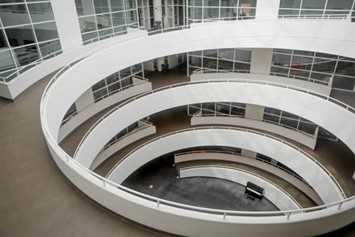
\includegraphics[height=5cm]{./images/spiral_groupt.jpg}
	\caption{The target environment for this project, Campus GroupT's spiral walkway (Leuven, Belgium).}
\end{figure}

\section{Sensors and MCUs}

Our project used the Bosch BNO055, a 9-axis intelligent absolute orientation sensor, and the BMP390, a high-precision barometric pressure sensor, for motion and altitude tracking, respectively. The BNO055 integrates a gyroscope, accelerometer, and magnetometer with an onboard microcontroller that fuses sensor data, offering orientation accuracy of  \textpm 1\textdegree \ in stable conditions.  \cite{bno055} Its self-calibrating features reduced the complexity of manual calibration, though environmental interference occasionally introduced noise. The BMP390 ensured altitude measurements in the precision of \textpm 0.03 hPa, thereby allowing for height estimations within a range of \textpm 0.25 meters. \cite{bmp390}

\begin{figure}[h] 
	\centering 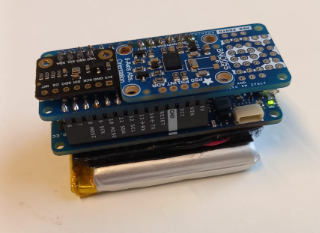
\includegraphics[height=5cm]{./images/hamburger.png}
	\caption{The Arduino module and sensors used.}
\end{figure}
	\chapter{Related Work}
The task of IMU-based head-tracking and positioning is a decades old task with significant literature exploring many different methods and solutions. A large portion of existing literature exploits knowledge of the system's behavioral model and multiple measurement sensors to implement Kalman filtering schemes \cite{sabatini_2011_kalmanfilterbased, hellmers_2013_an}. More recent methods also include step detection and counting methods in order to reduce drift issues in dead reckoning applications \cite{tiwari_2022_a, huang_2022_improvement}. Finally, with the modern advancements in compute and machine learning algorithms, machine learming methods have been implemented to create end-to-end solutions for position and orientation tracking using machine learning models and large labelled datasets. Additionally, using IMU data isn't the only proposed solution for cost-effective position tracking systems, with many system exploiting the ubiquity of WLAN/Wi-Fi to incorporate signal strength information into their system for additional positioning accuracy. \cite{stanculeanu_2012_enhanced, shang_2014_a}.
	\chapter{Methods and Implementations}

\section{Dataset Collection}
In order to evaluate and test the various schemes discussed in this paper, we conducted controlled experiments to capture and label head position and orientation data along the spiral path. Two primary data sources were utilized: sensor measurements, including data from a 9 Degrees of Freedom (DOF) sensor and a barometric pressure sensor, and network signals captured from routers at the target environment. Details regarding the collection and preprocessing of the dataset can be found in Appendix~\ref{appendix:dataset}.

\section{Synthetic Data Generation}
An additional synthetic data pipeline was implemented in order to achieve 3 main goals: providing an alternative to tedious data collection procedures, allowing for quick prototyping of algorithms and schemes before the full dataset was collected, and ensure behavioral integrity and reliability of implemented schemes before real evaluations. Since the required synthetic data generation was not meant to replace the actual dataset, we opted for a simple mathematical model for the sensor outputs, followed by sampled white gaussian noise.
\par
The implemented pipeline is able to generate artificial sensor readings for any given "ground truth" trajectory, whether that trajectory is actual collected data, or synthetically generated positions. Using a simple discrete derivative formula, the velocities and accelerations were calculated from the input positions, and the rotations were calculated as the tangents to the synthetic spiral. Following that, the pressure value is calculated using the altitude-pressure formula \cite{barometric} and white gaussian noise is added to the measurements.
\par
Furthermore, artificial Wi-Fi RSSI data was added to the synthetic data pipeline, using defined BSSIDs in certain positions, and the distance-RSSI formula. \cite{shang_2014_a} Finally, all this data is stored similarly to the actual dataset, in an identically formatted HDF5 sequence, to allow for interchangeability between the real and synthetic sequences.


\section{Position Estimation}
\subsection{Naive Double Integration Dead Reckoning}
The simplest and most well-known approach to positioning using IMU data is naive double integration dead reckoning (NDI) \cite{yan_2019_ronin}, where the acceleration components are discretely integrated into velocities, which are then in turn integrated into positions. The issue with this approach is that due to the double integration, sensor offsets, and noise can easily snowball due to the double integration procedure and as such the predictions drift very quickly. \cite{yan_2019_ronin}. In experiments with NDI, the algorithm's predictions went out of control very quickly. Due to these issues, NDI is not a solution for the indoor positioning problem.

\begin{figure}[h] 
	\centering 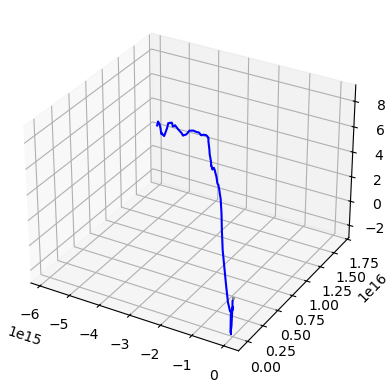
\includegraphics[height=5cm]{./images/ndi.png}
	\caption{The massive drift issues apparent in NDI.}
\end{figure}

\subsection{Pressure and Environment Model Based Positioning}
The next positioning method we explored was using the BMP390 pressure sensor's pressure values, along with our environment model for the spiral environment.
\subsubsection{Pressure Based Altitude Estimation}
Using the following formula, we determined the height values using the pressure data received.
$$P\left(z\right)=P_0e^{-\alpha z}$$

Using the derived pressure values, we calculate a 3D position in the target environment using a direct mapping from altitude values to 3D positions built on information about the target environment. Using information from both our ground truth data in our collected dataset, and ground plan data of the target environment. The mathematical model implements a mathematically ideal spiral, with its parameters tuned to best fit the ground truth data and the floor plan data. After visual tuning and comparing values with the ground plans, the parameters finally used are shown below, along with a diagram showing the ground truth data next to the model data.

\begin{figure}[h] 
	\centering 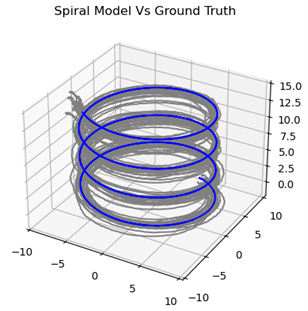
\includegraphics[height=5cm]{./images/spiralmodel.png}
	\caption{A visualization of the derived spiral model (blue) and the ground truth data (gray).}
\end{figure}

\begin{table}[h!]
\centering
\renewcommand{\arraystretch}{0.9} % Reduce row height
\setlength{\tabcolsep}{6pt}       % Reduce column spacing
\begin{tabular}{|l|c|}
\hline
\textbf{Parameter}       & \textbf{Value (m)} \\ \hline
\texttt{spiral\_pitch}   & 4.2               \\ \hline
\texttt{spiral\_radius}  & 8.0               \\ \hline
\texttt{path\_width}     & 2.4               \\ \hline
\end{tabular}
\vspace{-0.5em}
\caption{Parameters of the spiral model.}
\label{tab:spiral_params}
\end{table}
\par

The spiral mathematical model was furthermore developed with functionality to align them with ground truth data spirals, to allow for more accurate inference. This is done via calculating the maximum bounds along the x and y axes of the spiral, and then using the resulting centroid as the center of the spiral. Furthermore, the spiral model is capable of deriving a 3D position using a Z value using the formulas below.
$$\theta=2\pi\frac{z}{p}$$
$$x=x_0+r\cdot cos\left(\theta+\varphi\right)$$
$$y=y_0-\ r\cdot sin\left(\theta+\varphi\right)$$ 

Where theta is the angle on the circular top-down projection of the spiral, x, y, z are the 3D positions of the output point (and z is the input height), phi is the phase shift of the spiral calculated at alignment, r is the radius of the spiral, p is the pitch of the spiral, and $x_0$ and $y_0$ are the center x and y position of the spiral's top-down projection.
Additionally, the model is capable of calculating the closest point on the spiral model to an arbitrary input point. The distance between an arbitrary point and a point on the spiral was derived mathematically in cylindrical space, using $r_{sp}$, $h_{sp}$, and $\theta_{sp}$ as the position of the closest point on the spiral to the arbitrary point $r_{pt}$, $h_{pt}$, and $\theta_{pt}$. Then an optimization problem was solved by solving $d^2\prime$ = 0. The formulas for this problem are shown below

$$d^2=r_{sp}^2+r_{pt}^2-2r_{sp}r_{pt}cos\left(\theta_{sp}-\theta_{pt}\right)+\left(h_{sp}-h_{pt}\right)^2$$
$$\theta_{sp}=2\pi\frac{h_{sp}}{p}$$
$$\frac{{d(d}^2)}{d(h_{sp})}=\ \frac{4\pi r_{sp}r_{pt}}{p}sin(\frac{2\pi h_{sp}}{p}-\theta_{sp})+2h_{sp}-2h_{pt}$$

After the formula above was derived, finding a solution analytically was difficult, and solvers were unable to compute a solution due to the periodicity of the sine section of the formula. As a result, we opted for a polynomial half period approximation of a sine wave  and used a symbolic solver to derive the candidate solutions for the optimal point. There are 3 candidate solutions, we choose the solution that produces the lowest distance and return the point at the resulting $h_{sp}$. 

$$sin\ x\ \approx\ \frac{16x(\pi-x)}{5\pi^2-4x(\pi-x)}$$

\subsection{Wi-Fi Based Positioning}
Given the ubiquitous nature of Wi-Fi networks, using Wi-Fi data for positioning is a very attractive approach. Additionally, the target environment, being a university campus, was filled with constant position Wi-Fi networks, which could be used as anchors for a fingerprinting system. To this end, we implemented a random forest regressor model and trained it over our dataset in order to predict 3D positions using the detected BSSID to RSSI data measured from the Arduino's Wi-Fi module. \cite{pedregosa_2011_scikitlearn}
\par

The model's input format is a vector of RSSI values, with each position being associated with a unique Wi-Fi BSSID found in the training set. During inference, any BSSIDs not found in the dataset are disregarded, and any BSSIDs found have their associated RSSI values placed at the corresponding position in the input vector. Any undetected BSSIDs in the input vector are set to a value of -100dB.
\par

A grid search was conducted over the number of estimators and the maximum depth, and the following model hyperparameters were determined to perform best for our task. The results of the grid search are shown along with the model's hyperparameters in \cref{tab:model_hyperparameters}.
\par
\begin{table}[h!]
\centering
\renewcommand{\arraystretch}{1.1} % Adjust row height
\setlength{\tabcolsep}{8pt}       % Adjust column spacing
\begin{tabular}{|l|l|}
\hline
\textbf{Parameter}                 & \textbf{Value}             \\ \hline
\texttt{bootstrap}                 & True                       \\ \hline
\texttt{ccp\_alpha}                & 0.0                        \\ \hline
\texttt{criterion}                 & 'squared\_error'           \\ \hline
\texttt{max\_depth}                & 28                         \\ \hline
\texttt{max\_features}             & 1.0                        \\ \hline
\texttt{max\_leaf\_nodes}          & None                       \\ \hline
\texttt{max\_samples}              & None                       \\ \hline
\texttt{min\_impurity\_decrease}   & 0.0                        \\ \hline
\texttt{min\_samples\_leaf}        & 1                          \\ \hline
\texttt{min\_samples\_split}       & 2                          \\ \hline
\texttt{min\_weight\_fraction\_leaf} & 0.0                      \\ \hline
\texttt{monotonic\_cst}            & None                       \\ \hline
\texttt{n\_estimators}             & 525                        \\ \hline
\texttt{n\_jobs}                   & None                       \\ \hline
\texttt{oob\_score}                & False                      \\ \hline
\texttt{random\_state}             & None                       \\ \hline
\texttt{verbose}                   & 0                          \\ \hline
\texttt{warm\_start}               & False                      \\ \hline
\end{tabular}
\caption{Model Hyperparameters.}
\label{tab:model_hyperparameters}
\end{table}
\par

\subsection{Kalman Filtering Schemes}
Using a combination of the IMU's accelerometer data with the NDI method, and the BMP390's pressure data and the derived altitudes, we implemented our first Kalman filtering scheme, which fuses the data from these two sources to attempt to find a more accurate output. The Kalman filter was implemented with a state vector containing the positions and velocities along the x, y, and z axes. A mathematical formulation of the filter is shown below. These filters were then tuned by a scalar parameter scaling these matrices.
\par
\[
H_{\text{PRESSURE}} =
\begin{bmatrix}
1.0 & 0.0 & 0.0 & 0.0 & 0.0 & 0.0 \\
0.0 & 1.0 & 0.0 & 0.0 & 0.0 & 0.0 \\
0.0 & 0.0 & 1.0 & 0.0 & 0.0 & 0.0 \\
\end{bmatrix}
\]
\begin{center}
\textbf{Matrix 1:} Measurement matrix for pressure state variables.
\end{center}


\[
H_{\text{WIFI}} =
\begin{bmatrix}
1.0 & 0.0 & 0.0 & 0.0 & 0.0 & 0.0 \\
0.0 & 1.0 & 0.0 & 0.0 & 0.0 & 0.0 \\
0.0 & 0.0 & 1.0 & 0.0 & 0.0 & 0.0 \\
\end{bmatrix}
\]
\begin{center}
\textbf{Matrix 2:} Measurement matrix for WiFi state variables.
\end{center}


\[
A =
\begin{bmatrix}
1.0 & 0.0 & 0.0 & \Delta t & 0.0 & 0.0 \\
0.0 & 1.0 & 0.0 & 0.0 & \Delta t & 0.0 \\
0.0 & 0.0 & 1.0 & 0.0 & 0.0 & \Delta t \\
0.0 & 0.0 & 0.0 & 1.0 & 0.0 & 0.0 \\
0.0 & 0.0 & 0.0 & 0.0 & 1.0 & 0.0 \\
0.0 & 0.0 & 0.0 & 0.0 & 0.0 & 1.0 \\
\end{bmatrix}
\]
\begin{center}
\textbf{Matrix 3:} State transition matrix.
\end{center}

\[
B =
\begin{bmatrix}
0.5\Delta t^2 & 0.0 & 0.0 \\
0.0 & 0.5\Delta t^2 & 0.0 \\
0.0 & 0.0 & 0.5\Delta t^2 \\
\Delta t & 0.0 & 0.0 \\
0.0 & \Delta t & 0.0 \\
0.0 & 0.0 & \Delta t \\
\end{bmatrix}
\]
\begin{center}
\textbf{Matrix 4:} Control transition matrix.
\end{center}

\par
The filter's covariance and noise matrices were tuned by hand and evaluated over dataset sequences in order to choose the best performing values.
\par
Another architecture we experimented with was incorporating the Wi-Fi positioning data as well into the Kalman filtering scheme. This Kalman filter used the same state vector and transition matrix, however, the filter was updated using both the pressure-altitude based positions and the Wi-Fi positioning data.

\section{Orientation Estimation}
The second step of the head-tracking system was implementing an attitude estimation system. Our implemented attitude system uses the BNO055 IMU's orientation estimation system, with some further postprocessing. The data is retrieved as roll, pitch, yaw Euler angles in degrees, and are baselined on an initial assumption of the user starting approximately at the orientation origin. \cite{bno055}

\section{Real-Time Communication}
The final step of the head-tracking system was ensuring the system can run in real-time and not just on the collected dataset. Given that our signal processing schemes were implemented to run in a python desktop environment and were incapable of running on the microcontroller, we had to set up real-time network communication between the system and the python environment. We implemented two interchangeable communication layers; one built on TCP, and one built on UDP. The UDP system is preferred and was used for our data collection and real-time testing, since the system is more efficient and robust to packet drops. The system relies on two internal data structures used to represent the sensor data and the Wi-Fi data respectively.
\par

 \noindent\small
\begin{table}[h!]
\centering
\resizebox{\linewidth}{!}{ % Resize table to fit column width
\begin{tabular}{|l|l|l|l|}
\hline
\textbf{Type}            & \textbf{Name}                     & \textbf{Size (bytes)}   & \textbf{Notes}              \\ \hline
\texttt{unsigned long}   & \texttt{microsT}                  & 4                      & 4 bytes padding             \\ \hline
\texttt{double}          & \texttt{linaccelx, linaccely, linaccelz} & $8 \times 3 = 24$ & Linear acceleration         \\ \hline
\texttt{double}          & \texttt{gyrox, gyroy, gyroz}      & $8 \times 3 = 24$      & Gyroscope values            \\ \hline
\texttt{double}          & \texttt{magnx, magny, magnz}      & $8 \times 3 = 24$      & Magnetometer values         \\ \hline
\texttt{double}          & \texttt{roll, pitch, yaw}         & $8 \times 3 = 24$      & Orientation values          \\ \hline
\texttt{int8\_t}         & \texttt{tempnbo}                  & 1                      & 7 bytes padding             \\ \hline
\texttt{double}          & \texttt{tempbmp}                  & 8                      & Temperature                 \\ \hline
\texttt{double}          & \texttt{pressure}                 & 8                      & Pressure                    \\ \hline
\end{tabular}
}
\caption{Structure of \texttt{DataEntry} (Size: 128 bytes).}
\label{tab:dataentry}
\end{table}

\noindent\small
\begin{table}[h!]
\centering
\resizebox{\linewidth}{!}{ % Resize table to fit column width
\begin{tabular}{|l|l|l|l|}
\hline
\textbf{Type}            & \textbf{Name}               & \textbf{Size (bytes)}   & \textbf{Notes}              \\ \hline
\texttt{unsigned long}   & \texttt{microsT}            & 4                      & -                           \\ \hline
\texttt{int8\_t}         & \texttt{rssiCnt}            & 1                      & 1 byte padding              \\ \hline
\texttt{byte}            & \texttt{BSSIDs[25][6]}      & $25 \times 6 = 150$    & 1 byte padding              \\ \hline
\texttt{int32\_t}        & \texttt{RSSIs[25]}          & $25 \times 4 = 100$    & -                           \\ \hline
\end{tabular}
}
\caption{Structure of \texttt{RssiDataEntry} (Size: 256 bytes).}
\label{tab:rssidatadataentry}
\end{table}

\par

\section{Visualization}

To visualize data in real-time, we initially used matplotlib's Animation module for simple animations to validate our solution. However, due to its limitations, we switched to Blender, a free 3D graphics software known for realistic 3D rendering, camera, lighting, and material options, and Python scripting capabilities. 
We first animated the ground truth and unfiltered data in Blender, using the data from h5 files. Once confirmed to be working as expected, we modeled the real-time data from our implementation.
\par
Blender includes its own Python environment, requiring the installation of necessary Python libraries within Blender's Python. Since the filtering script and Blender visualization ran in separate Python environments, we established communication between them using TCP sockets. The main Python script acted as a server, sending orientation and position data to the Blender script, which acted as a client, receiving the data.
\par
We modeled the spiral, floor, and walls in 3D, adding lighting and camera tracking. In the final Blender file, a face is visible in the main frame, adjusting the camara to follow along the spiral as a person ascends.
Blender on our PCs could render at a maximum of 25 frames per second (fps), while our solution sampled at 100Hz. To synchronize the visualization with real-time position and orientation, we sent only one sample of position and orientation data out of every four samples to the Blender script.
\cref{viz} displays the final Blender animation. On the right is the camera view, focusing on the monkey face at the center. On the left is a overview visualization of all the objects that were modeled.

\begin{figure}[h] 
	\centering 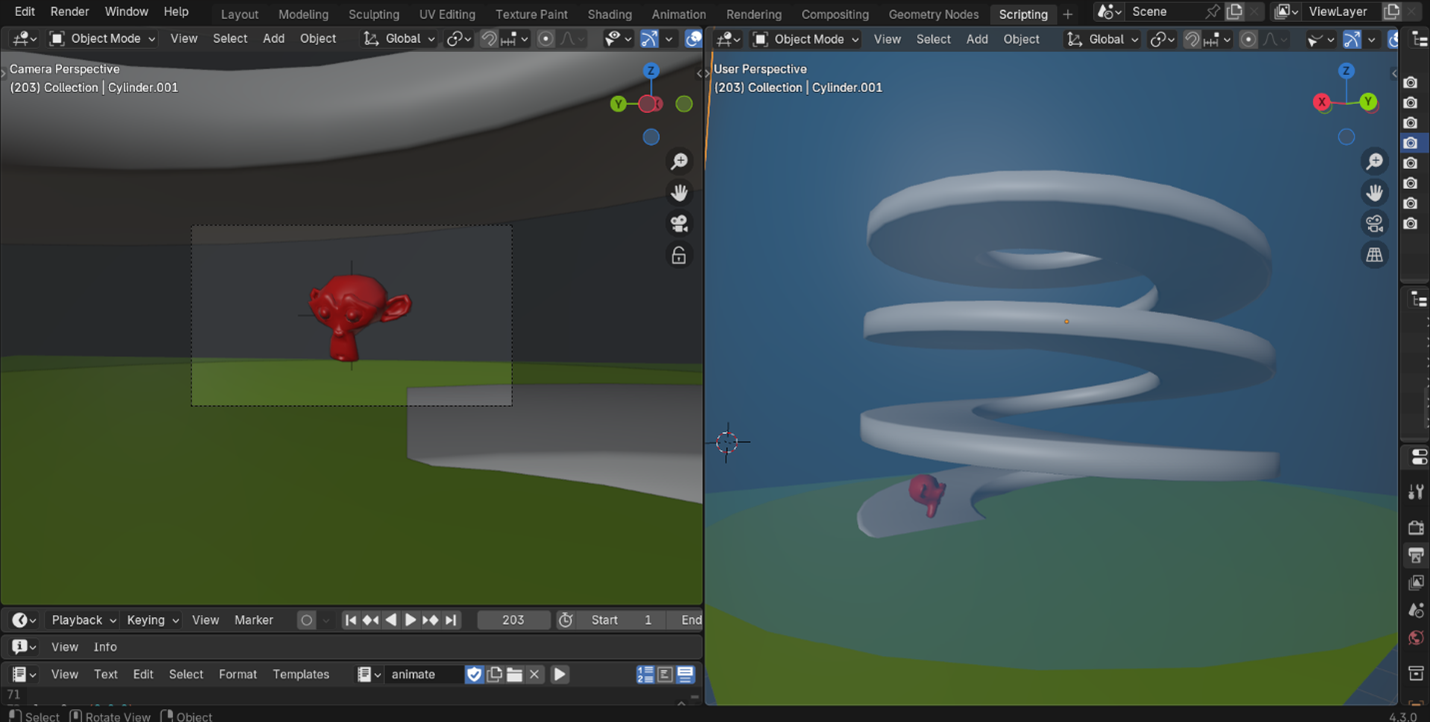
\includegraphics[height=4cm]{./images/visualization.png}
	\caption{A preview of the implemented visualizer.}
	\label{viz}
\end{figure}


	\chapter{Results and Evaluation}
In order to assess the quality and performance of the proposed systems, we ran various qualitative and quantitative evaluations. The results of these evaluations are presented below.

\section{Hardware Limitations}
Our first plan was to run the Kalman filter on the Arduino itself. This proved challenging since the filter requires a lot of computation and we had doubts on the performance of Arduino with the filter on producing real time results. To that end, we implemented a simple Kalman filter that did not integrate all the aspects of the real filter in order to address the hardware limitation, which worked well but did not achieve our expected performance or results. The Arduino MKR 1010 is not designed for computationally intensive tasks like matrix multiplication. Small matrices (e.g., 3x3 or 4x4) can be handled reasonably, but as matrix sizes grow, performance drops significantly due to limited processing power and memory. NumPy uses highly optimized libraries like BLAS and LAPACK. These libraries leverage multi-threading, SIMD instructions, and efficient memory access patterns to maximize speed. The performance scales well with larger matrices.\cite{hellmers_2013_an} To that end, we decided to implement the complete Kalman filter in Python and we would transfer the sensor reading from the Arduino to a Laptop to process it.

\section{Positioning Systems}
\subsection{Wi-Fi Data Random Forest Regressor}
The Wi-Fi RFR model was evaluated on average error, max error, mean squared error, and R2 score in order to show various aspects of the model's behavior.
\begin{table}[h!]
\centering
\caption{Error Metrics for Test and Unseen Sets}
\label{tab:error_metrics}
\begin{tabular}{l c c} % Left, Center, Center alignment
\toprule
\textbf{Metric}                  & \textbf{Test Set} & \textbf{Unseen Set} \\ 
\midrule
Average Error (m)                & 6.47              & 6.93                \\
Max Error (m)                    & 9.27              & 11.33               \\
Mean Squared Error (m\textsuperscript{2}) & 43.9              & 49.7                \\
R\textsuperscript{2} Score       & 0.536             & -                   \\ 
\bottomrule
\end{tabular}
\end{table}

A qualitative sample of the RFR model running on a single data sequence is seen below, showing the Wi-Fi model's predictions in orange, and the ground truth positions in blue.
\begin{figure}[h] 
	\centering 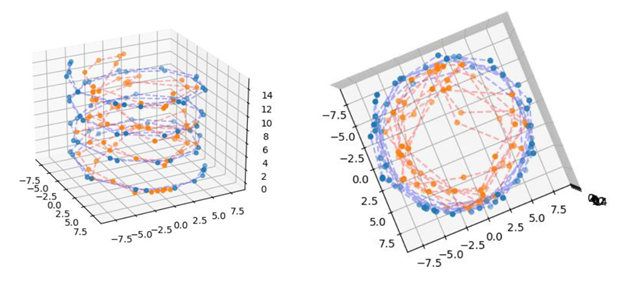
\includegraphics[height=4cm]{./images/wifirf.png}
	\caption{An example of the Wi-Fi RFR Model's predictions (orange) and  the ground truth path (blue).}
\end{figure}

\subsection{Kalman Filtering Schemes}
In the evaluation of the positioning system, three main metrics were used: the absolute trajectory error (ATE), relative trajectory error (RTE), and the average error. \cite{rtabmap, yan_2019_ronin} The implemented evaluations were implemented with a linear interpolation system, in order to be able to evaluate the metrics over two signals with different sample times.

\begin{table}[h!]
\centering
\caption{Trajectory and Average Errors Using Different Methods}
\label{tab:trajectory_errors}
\setlength{\tabcolsep}{3pt} % Adjust column spacing
\small % Reduce font size slightly to fit content
\begin{tabularx}{\columnwidth}{l X X X} % X columns for auto-adjust
\toprule
\textbf{Metric} & \textbf{Pressure Only} & 
\textbf{\centering Kalman Fusing Accelerometer and Pressure} & 
\textbf{Kalman with Wi-Fi Data} \\ 
\midrule
ATE (m) & 3.28 & 3.28 & 5.54 \\
RTE (m) & 3.01 & 3.01 & 3.07 \\
Average Error (m)             & 2.25 & 2.25 & 4.07 \\
\bottomrule
\end{tabularx}
\end{table}

\section{Orientation Estimation System}
To evaluate the orientation system, we used average, median, and max error as evalution metrics. Furthermore, we evaluated the system both as a whole and on individual angle components.

\begin{table}[h!]
\centering
\caption{Error Metrics in Degrees}
\label{tab:single_value_metrics}
\setlength{\tabcolsep}{36pt} % Adjust column spacing
\small % Reduce font size
\begin{tabularx}{\columnwidth}{l c} % Left-aligned and center columns
\toprule
\textbf{Metric}      & \textbf{Value (\textdegree \ )} \\ 
\midrule
Median Error         & 35   \\
Average Error        & 39   \\
Max Error            & 162  \\ 
\bottomrule
\end{tabularx}
\end{table}

\begin{table}[h!]
\centering
\caption{Error Metrics for Roll, Pitch, and Yaw}
\label{tab:roll_pitch_yaw_errors}
\setlength{\tabcolsep}{10pt} % Adjust column spacing
\small % Reduce font size
\begin{tabularx}{\columnwidth}{l c c c} % Left and center columns
\toprule
\textbf{Metric}      & \textbf{Roll (\textdegree \ )} & \textbf{Pitch (\textdegree \ )} & \textbf{Yaw (\textdegree \ )} \\ 
\midrule
Median Error         & 34.39                   & 3.75                    & 2.40                  \\
Average Error        & 38.61                  & 4.09                    & 2.84                  \\
Max Error            & 162.46                 & 21.50                   & 18.21                 \\ 
\bottomrule
\end{tabularx}
\end{table}

Furthermore, a qualitative sample of a single sequence is shown below. In this sequence, the heading (roll) is represented by the red signals, and the pitch and yaw are represented as the blue and gray signals.

\begin{figure}[h] 
	\centering 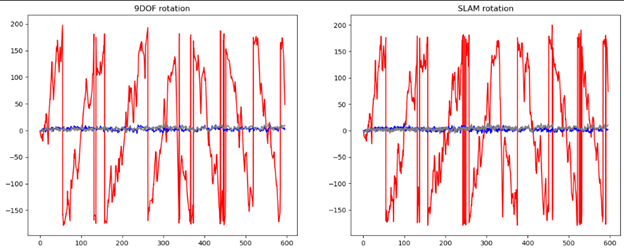
\includegraphics[height=3cm]{./images/rotations.png}
	\caption{The measured (left) and ground truth (right) rotation values with heading, pitch, and yaw in red, gray, blue respectively.}
\end{figure}



	\chapter{Discussion}

\section{Positioning Systems}
In terms of pure performance, the pressure-based system heavily outperforms every other proposed system, barring the Kalman filtering schemes tuned to prioritize pressure data. This is due to the high accuracy and sampling rate of the pressure data in our system, which when combined with the well-tuned altitude based mathematical spiral model, allows us to calculate accurate positions at a very high sampling rate. Due to this, the noisy data from the accelerometers and the Wi-Fi RFR weren't able to improve the predicted positions significantly. However, the constraints placed on the system in terms of the target environment are difficult to generalize to other use-cases, where a system relying only on pressure data wouldn't be able to determine the X and Y positions with a reasonable accuracy.
\par
Furthermore, if the spiral model used was mistuned or if the alignment was imperfect, the accuracy of the pressure-based system suffers significantly, which we encountered during our tuning. In cases where the environment model cannot deterministically predict an X, Y position for a given height, or in cases where the environment model is inaccurate or inconsistent, the Wi-Fi based Kalman filtering scheme can provide an additional layer of error correction and outperforms the pressure-only system. Furthermore, the entire pressure system heavily relies on the prior knowledge of the pressure at the starting position, which may not be known in some environments, or may vary. To deal with this, a separate module can be placed at a baseline position, in order to collect the pressure at the ground. An alternative method is to rely further on the Wi-Fi fingerprinting system, which does not rely on a predetermined pressure baseline value.

\section{Orientation Estimation Systems}
The orientation system proposed appears to perform well from a distance, with generally accurate orientation values along entire sequences. However, the system is prone to occasional drift issues, specifically on the heading axis. This is due to two main reasons. Firstly, the heading axis lacks an accurate baseline in the form of the gravity vector, which is only available on the other two axes. This issue can be mitigated via integrating a more accurate sensor or implementing a Kalman filtering/machine learning scheme to further improve the predicted angles. Secondly, the heading axis exhibits significantly larger variance than the other two axes of rotation, simply due to human anatomy and range of motion. However, the orientation estimation system generally performs well, with below 30 degrees of median angular error.
	\chapter{Future Work}

\section{Sensors and MCUs}

A proposed alternative to the Arduino MKR1010 is an upgrade to an ESP32 device. An ESP32-WROOM-32 upgrade offers serious improvements over the Arduino MKR1010 in applications needing efficient processing, reduced latency, and energy savings. ESP32 outperforms MKR1010 with a dual-core 240 MHz processor, as opposed to MKR1010's single-core 48 MHz, and a larger RAM capacity of 520 KB against 32 KB. The increased computational power of the ESP32 enables it to do some real-time computations, like running Kalman filters, onboard without the use of an external computer. This removes the high latency and network dependency associated with the MKR1010-based method, where sensor data has to travel to a laptop for processing.
\par
The ESP32 also boasts significantly improved connectivity capabilities that include Wi-Fi and Bluetooth v4.2/BLE. With its dual-mode Wi-Fi operation (STA + AP), the ESP32 allows asynchronous network scanning without interrupting the active connections, which the MKR1010 cannot do. This allows for continuous data transmission while keeping the power consumption low by using intermittent Wi-Fi.
\par
Also, it reduces the system complexity since the ESP32 eliminates the use of external PCs, making deployment and integration easier. The performance and scalability increase because of its capability to handle real-time updates on its own. At a lower cost of ~\$5-10 with more I/O pins, 36 compared to 22, the ESP32 presents an economical, high-performance solution.
\par
Among several conclusions, it is considered that the migration to the ESP32-WROOM-32 avoids limitations concerning latency, energy usage, and system complexity brought into perspective by MKR1010, adding computational efficiency that makes this board definitely superior for real-time application employment. \cite{brownlee_2023_numpy}

\section{Synthetic Data Generation}
In order to improve the quality of our synthetic data so it better mimics real life data, there are several things that can be improved.
Firstly, the velocity equation used, and trajectory could be improved to be more complex and to be better mimic real-life velocity and trajectory of a person going up a spiral. However, since these are modeled by mathematical equations, they cannot model the random behavior of human behavior. 
\par
Another adjustment would be to better model the noise added by the different sensors. In the datasheet, the average and the standard deviation of said noise is mentioned because it can be modeled as additive white gaussian noise, however in real life noise generated by the sensor might be more complex. To add noise to our synthetic data that can more accurately copy real-life noise created by the sensors, deep learning can be used. 
\par
Generative AI can help create realistic sensor noise. By training on a dataset collected from still sensors - where acceleration is zero and pressure, gravity, and the magnetic field are constant - Generative AI could replicate the noise profile. To account for variability due to factors like temperature or sensor orientation, data collection should be repeated on different days and in different positions. 
\cite{tang_2024_synthetic} describes creating a synthetic IMU dataset simulating a person falling. The dataset was trained using SLAM data recorded in an environment free from occlusions. Similarly, we could collect SLAM and IMU data to isolate sensor noise and use it to train a model capable of generating highly realistic IMU noise. In \cref{LSTM_synthdata} the structure of the LSTM model used to generate synthetic data can be seen and \cref{setup_sythndata} shows the experimental set up used.
\begin{figure}[h] 
	\centering 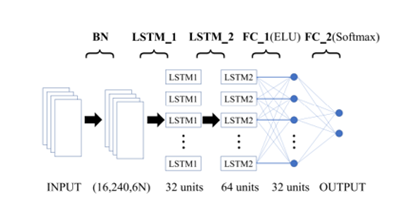
\includegraphics[height=4cm]{./images/LSTMsynth.png}
	\caption{The LSTM architecture used for generating the synthetic data.}
	\label{LSTM_synthdata}
\end{figure}
\begin{figure}[h] 
	\centering 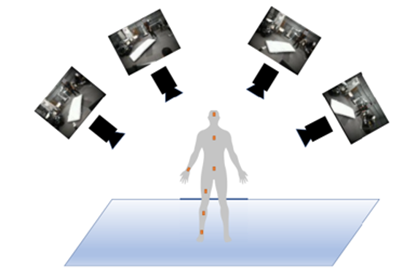
\includegraphics[height=4cm]{./images/setupsynth.png}
	\caption{The experimental setup used for generating the synthetic data.}
	\label{setup_synthdata}
\end{figure}

\section{Data Collection and Processing}
For the future there are several points to improve upon both for data collection and pre-processing. 
For Data collection:

\begin{itemize}
  \item Data collection could be done using more accurate SLAM tools instead of an iPhone. An example of such a tool would be a high-quality stereo camera with LIDAR. This would help improve the accuracy of the data measured.
  \item Generate synthetic variations of the collected dataset to simulate different scenarios. So, using data augmentation, we would create different datasets from an originally measured one to increase and vary our dataset.
\end{itemize}

For pre-processing:

\begin{itemize}
  \item As mentioned before, the method used for synchronization of the ground truth and the raw data was not perfect as it was coarse tuning. Therefore, a fine-tuning method can be applied. This first starts by resampling one of the two signals so that they both have the same sampling frequency. This is crucial because the next step is performing the cross correlation of the signals, and to do that, the signals should have a constant and equal sampling frequency. Performing the cross correlation informs us of how much the 2 signals lag each other, and we can then shift one of the signals by that time to match them. This will help synchronize the signals properly. \cite{yan_2019_ronin}
\end{itemize}

\section{Position Estimation}
The implemented positioning system can be improved via various methods, however, given the scope and requirements of the project, we propose a few main future improvements to the system. 

Firstly, a major issue facing the positioning system, is the inaccuracies of the mathematical spiral model. In order to improve this aspect of the system, a machine learning model can be trained in order to predict positions along the spiral more accurately than a constant mathematical model, and can better reflect the inconsistencies and intricacies of the ground truth data.

Secondly, another issue the system faces, is the lack of usefulness of the accelerometer data due to the high noise levels which causes excessive drift. To combat this, a common method explored in the literature is step counting, which employs situational assumptions about human movement in order to more accurately apply dead reckoning based positioning using IMU data. To implement this, an imu would need to be rigidly attached to the foot of the user ideally, however if this was infeasible, methods attempting step counting using head-attached IMUs can be explored. \cite{huang_2022_improvement, tiwari_2022_a}
Thirdly, the implemented simple Kalman filtering scheme fails to capture non-linear behavior exhibited by the system, and so implementing an Unscented Kalman filter \cite{bernalpolo_2019_kalman} can improve the performance of the system by improving the system's robustness to non-linear effects.

Finally, a trivial improvement which can be implemented to increase the performance of the overall system, is to replace the used sensors with better performing consumer grade sensors. As an example, the BNO085 is a similar IMU to the used BNO055 with better performance, and within the same price range.


\section{Orientation Estimation}
Future work in terms of the orientation estimation mainly should focus on improving the heading axis accuracy. The heading axis faces the largest issues in performance as seen in our evaluations, which is due to the two reasons discussed earlier. Resolving the issues due to the lack of a baseline vector in the form of the gravity vector will mainly involve implementing a more accurate baseline system based on magnetometer data or integrating different sensors that allow for accurate measurements on the heading axis. An example of this could be integration of spatially spaced sensors, and employing time-difference-of-arrival (TDoA) methods to measure the heading angle. \cite{stanculeanu_2012_enhanced} Furthermore, machine learning methods can be employed in order to improve prediction fidelity, and to learn non-trivial patterns from the dataset. \cite{yan_2019_ronin}


	\chapter{Conclusion}
In summary, the project successfully developed a robust real-time position and attitude estimation system tailored for the constrained indoor environment of KU Leuven's Group T Campus spiral walkway. The work implemented several techniques, such as altitude-based pressure models, Kalman filtering schemes, and machine learning approaches like Random Forest Regression, by fusing sensors with the Bosch BNO055 IMU, BMP390 pressure sensor, and Wi-Fi-based positioning. While the pressure-based system was the most accurate for vertical positioning, the Wi-Fi integration and Kalman filters did improve the accuracy in complex conditions. The attitude estimation, while reliable, had issues such as drift in the heading axis because of the inherent limitations in the IMU-based measurements.
 
Future work is directed at both hardware and algorithm improvements. For example, moving to more powerful microcontrollers, such as the ESP32, would support on-device processing and decrease latency and system complexity. Other improvements involve refining the generation of synthetic data, enhancing synchronization during preprocessing, and using higher-order positioning techniques, such as step counting and machine learning-driven spiral alignment. These improvements are aimed at solving current limitations, enhancing generalizability, and ensuring the robustness of the system in various real-world applications.



	%%% Bibliography: references. included from bibliography.bib
	%%% Only referenced items are displayed in the final document
	\nocite{*}			% if you also want to display the unreferenced items in your bibliografy uncomment this
	\bibliographystyle{ieeetranN}
	\bibliography{bibliography}

	%%% appendices
   %\appendix
    %\appendixpage
	%% when you are using the twocolumn layout for your thesis appendixes may/can be in a 'singlecolumnsection'
\begin{singlecolumnsection}
\end{singlecolumnsection}

	%%% Apendix from other pdf
%	\chapter{Poster}
%	\includepdf{poster.pdf}

	\backcover
\end{document}
